\namedsection{Ausgangssituation}{J}
Grundsätzlich ist die Vorgabe Daten aus Drittsystemen anzubinden indem eine API für die Anwendung von Statistance bereit gestellt wird. Diese Lösung sollte im Idealfall nicht nur leicht um weitere Anbindungen für Drittsysteme erweiterbar sein, sondern im Falle einer Cloud-Lösung mit zunehmenden Kunden gut skalieren.

\begin{figure}[!h]
\centering
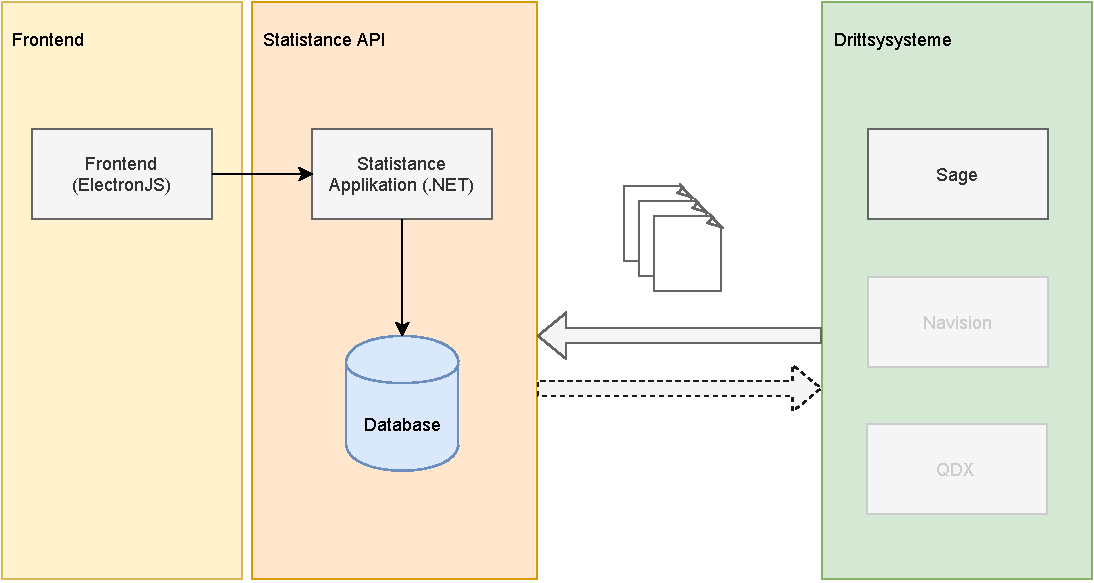
\includegraphics[width=8.5cm]{images/0x_requirement_analysis/statistance_ausgangssituation.pdf}
\caption{Ausgangssituation}
\end{figure}

Eine gute Lösung wäre in diesem Fall das bereits vorhandene Open Integration Hub gewesen, welches allerdings aus unterschiedlichen Gründen in der derzeitigen Form für Statistance nicht rentabel ist. Mehr über die Gründe können im Abschnitt über die Architektur erfahren werden oder im Vergleich unserer Lösung mit der vom Open Integration Hub.


Demzufolge hat sich der Geltungsbereich unsereres Projektes vor allem auf die gegenwärtigen Herausforderungen des Pilotkunden erstreckt. Namentlich die Integration von Sage 100, dass beim Pilotkunden in Benutzung ist. Darüber hinaus lag der Fokus auf eine On Premise Lösung. In Zukunft könnte der Kunde zudem auf eine aktuellere Sage Version umsteigen. Demzufolge sollte die Lösung auch erweiterbar sein.